% (Separate analysis.tex file, so all images are in a separate file.)

First, we verify that the simulation's output matches obviously expected
results. Then, we investigate aspects of its behavior which are not computable
analytically in order to discover important consequences of the model.


\subsection{Verification}

\subsubsection{Single simulation runs}

For a sensible range of parameter settings, the life history of a single
simulation run follows an expected pattern. Assuming a positive growth rate
(\textit{i.e.}, salary > metabolic rate), each agent's wealth rises unsteadily
during stage 1, until eventually the first pair of neighboring agents who each
reach the threshold form a proto-institution. Throughout stage 2, these agents
contribute all wealth in excess of the threshold to that proto, and so their
proto's balance rises unsteadily while their personal wealth remains at the
constant threshold. Meanwhile, the other agents also reach the threshold at
various points in time, and also form or join protos, until every non-isolate
(that is, every node with at least one neighbor) is a member of a proto. Stage
3 (the starvation period) then commences, with isolates drawing on a greater
personal wealth than the non-isolates. When an isolate reaches zero wealth, it
dies; when a non-isolate reaches zero, it draws from its (shared) proto balance
until that too, reaches zero, and it dies.

\begin{figure}[ht]
\centering
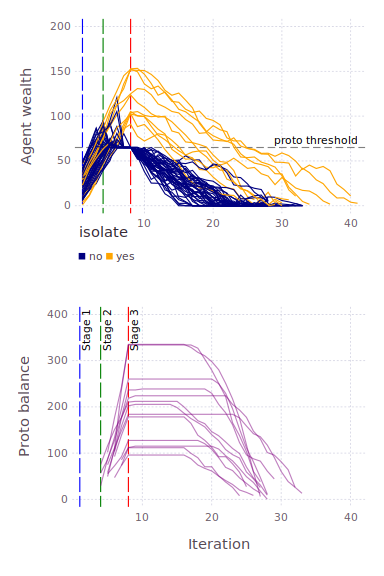
\includegraphics[width=\columnwidth]{figures/sampleLifeHistory.png}
\caption{A single run of the simulation, with $\lambda$=2. Each of 50 nodes is
given an initial wealth of $\sim\mathcal{U}(0,50)$ units, a regular income
distributed as $\sim\mathcal{N}(20,5)$, a metabolic rate of 5, and a proto
threshold of 65.} \label{fig:singleRun}
\end{figure}

This history can be seen in Figure~\ref{fig:singleRun}. The top plot depicts
agent wealth at every iteration, and the bottom plot shows the balances of the
protos at the same points in time. (No protos exist until stage 2, by
definition.) Note that the isolates (orange lines) never form protos, and
therefore begin the starvation stage with a higher personal wealth to draw
from.


\begin{figure}[ht]
\centering
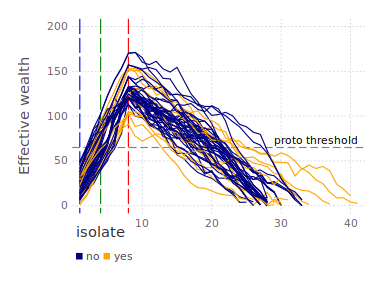
\includegraphics[width=\columnwidth]{figures/sampleEffectiveHistory.png}
\caption{The same simulation run as Figure~\ref{fig:singleRun}, but this time
depicting each agent's \textit{effective} wealth (its personal wealth plus its
share of its proto's wealth, if any).}
\label{fig:effectiveWealthSingleRun}
\end{figure}

Figure~\ref{fig:effectiveWealthSingleRun} shows the same information in another
way: instead of plotting each agent's \textit{personal} wealth (as in the top
plot of Figure~\ref{fig:singleRun}), we show its \textbf{effective wealth},
defined as the sum of its personal wealth and its ``share'' of its proto's
wealth (if any). After all, contributions that a proto's members make to its
balance are available to those members in times of need; therefore, a fair
comparison between isolates and non-isolates should take this into account.
From the figure, it can be seen that isolates no longer have a systematic
advantage (as they appeared to in Figure~\ref{fig:singleRun}.)

We verified that changes to basic parameters all have the expected effect:
lowering the initial wealth delays the onset of stage 2; a higher $\sigma^2$
for the income distribution makes the lines less jagged; a higher metabolic
rate hastens extinction; \textit{etc.}

To see how wealth inequality plays out over time, we plot the Gini coefficient
of the population in Figure~\ref{fig:giniHistory}. (The Gini calculation is
taken with respect to each agent's \textit{effective} wealth, not merely its
personal wealth.) In stage 2, we see inequality decrease as agents join one
another in protos and contribute their ``excess'' wealth to a shared pool. When
the stage 3 starvation period commences, inequality rises as the poorer agents
drop to zero and begin to deplete proto balances.

\begin{figure}[hb]
\centering
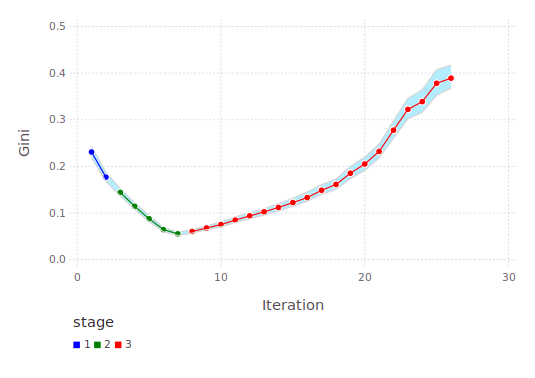
\includegraphics[width=\columnwidth]{figures/giniHistory.png}
\caption{The simulated society's wealth inequality over time. (The same
simulation parameters were used as in Figures~\ref{fig:singleRun} and
\ref{fig:effectiveWealthSingleRun}, but this time with 500 agents.)}
\label{fig:giniHistory}
\end{figure}

% Note that the empty graph can't really be shown because stages 2 and 3 have
% no well-defined meaning in that case.

% Show Gini plot, null hypothesis, "this is why it doesn't matter"

% Show different levels of white noise intensity relative to growth rate
%     (salary - metabolic rate)


\subsubsection{Parameter sweeps}

% Gini coefficient (pre-stage-3) decreases with λ

\subsection{Findings}

% Wealth histogram is steady ?

% Which is better strategy: to form protos when possible, or not?
